\begin{figure}[t]
    \centering
    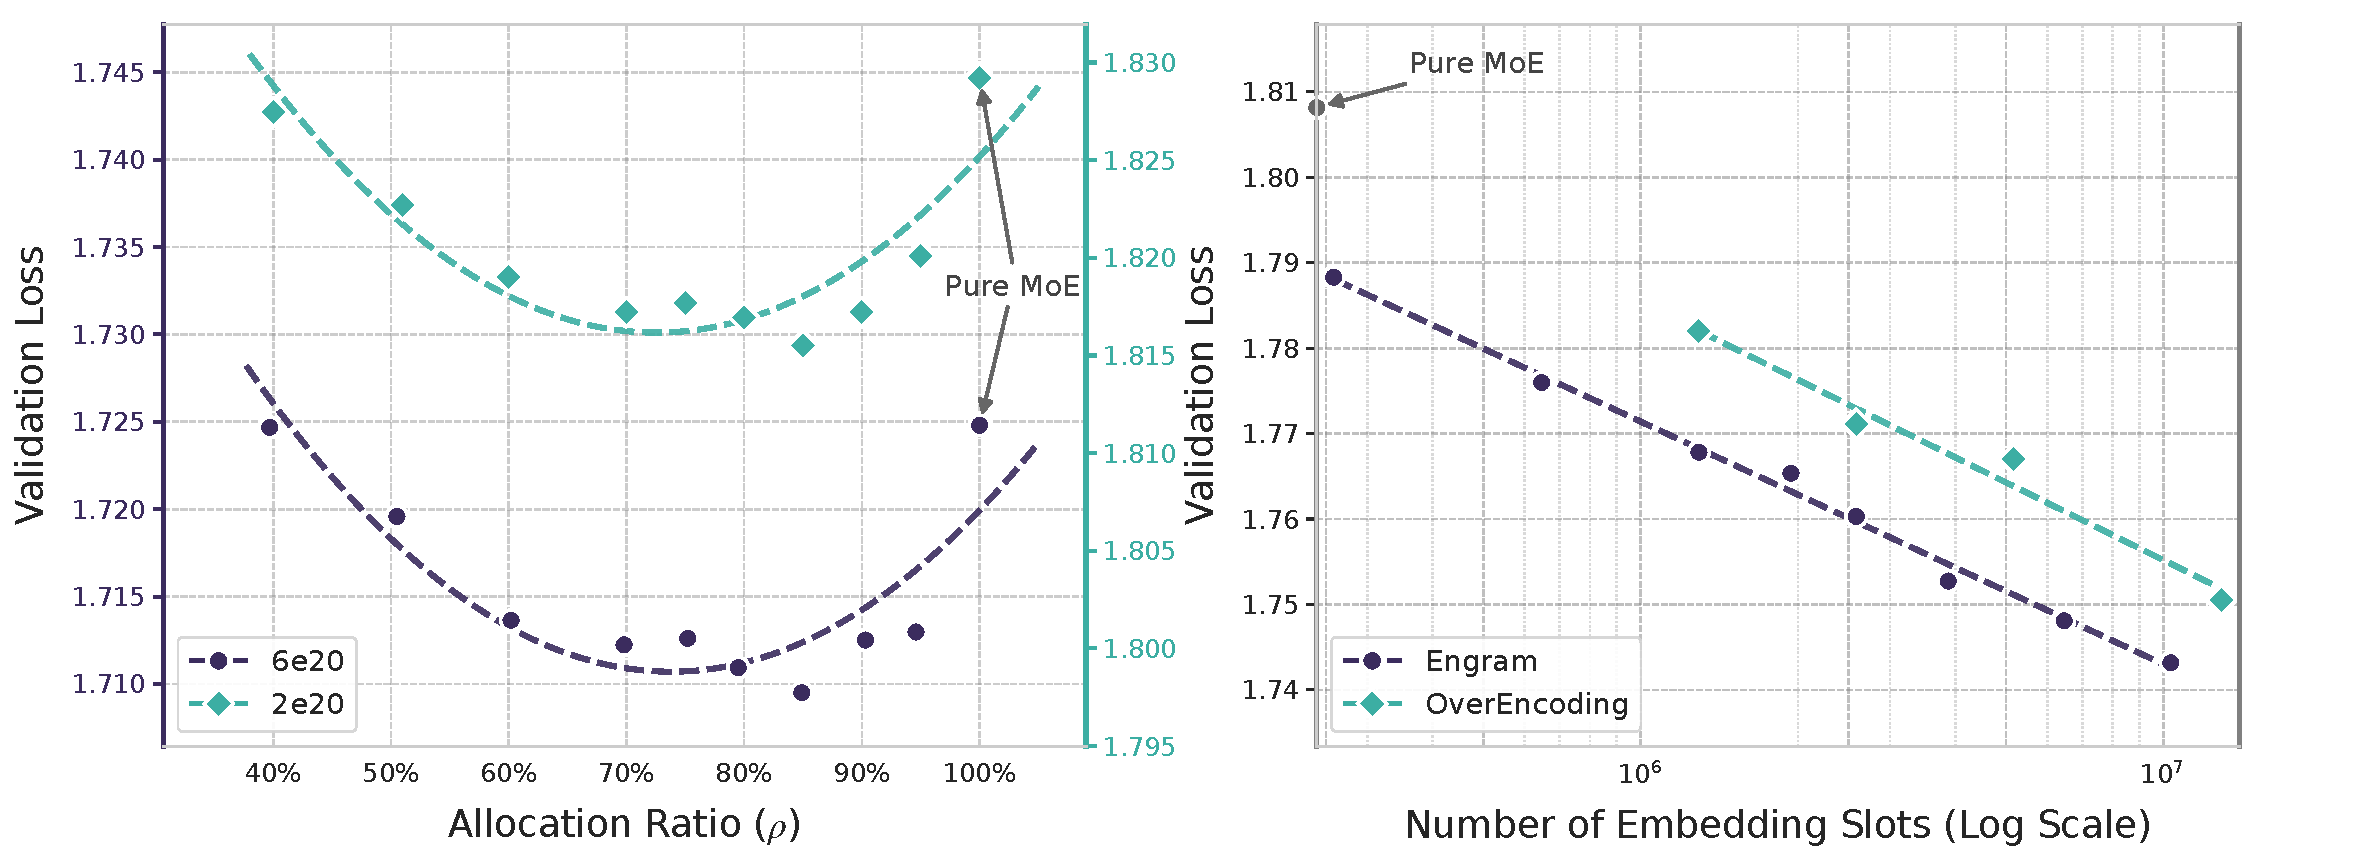
\includegraphics[width=0.95\linewidth]{figs/scaling_law.pdf}
    \caption{\textbf{Sparsity allocation and Engram scaling.}
        Left: Validation loss across allocation ratios $\rho$. Two compute budgets are shown ($2\text{e}20$ and $6\text{e}20$ FLOPs). Both regimes exhibit a U-shape, with hybrid allocation surpassing Pure MoE.
        Right: Scaling behavior in the infinite-memory regime. Validation loss exhibits a log-linear trend with respect to the number of embeddings.
    }
    \label{fig:scaling_law}
\end{figure}

\section{Scaling Laws and Sparsity Allocation}
\label{sec:scaling_law}

Engram, as an instantiation of conditional memory, is structurally complementary to the conditional computation provided by MoE experts.
This section investigates the scaling properties of this duality and how to optimally allocate sparse capacity. Specifically, two key questions drive our research:
\begin{enumerate}[leftmargin=*,itemsep=2pt,topsep=2pt]
    \item \textbf{Allocation under Finite Constraints.} When total parameters and training compute are fixed (Iso-parameter and Iso-FLOPs), how should we split the sparse capacity between MoE experts and Engram embeddings?
    \item \textbf{Infinite Memory Regime.} Considering the non-scaling $\mathcal{O}(1)$ overhead of Engram, if the memory budget is relaxed or scaled aggressively, what scaling behavior does Engram exhibit by itself?
\end{enumerate}

\subsection{Optimal Allocation Ratio Between MoE and Engram}
\label{sec:ratio_scaling_law}

\paragraph{Compute-matched formulation.}
We analyze the trade-off using three parameter metrics:
\begin{itemize}[leftmargin=*,itemsep=2pt,topsep=2pt]
    \item $P_{\mathrm{tot}}$: total trainable parameters, excluding vocabulary embedding and LM head.
    \item $P_{\mathrm{act}}$: activated parameters per token. This quantity determines the training cost (FLOPs).
    \item $P_{\mathrm{sparse}} \triangleq P_{\mathrm{tot}} - P_{\mathrm{act}}$: the \textit{inactive} parameters, which represents the ``free'' parameter budget available for scaling model size without incurring computational cost~(e.g., unselected experts or unretrieved embeddings).
\end{itemize}
We keep $P_{\mathrm{tot}}$ and $P_{\mathrm{act}}$ fixed within each FLOPs budget, so that models have the same number of parameters and the same per-token FLOPs. For MoE, $P_{\mathrm{act}}$ is determined by the top-$k$ selected experts, while the parameters of non-selected experts contribute to $P_{\mathrm{sparse}}$. For Engram, only a constant number of slots are retrieved per token, so scaling the number of embedding slots increases $P_{\mathrm{tot}}$ without increasing per-token FLOPs.


\paragraph{Allocation ratio.}
We define the allocation ratio $\rho\in[0,1]$ as the fraction of the inactive-parameter budget assigned to MoE expert capacity:
\begin{equation}
P_{\mathrm{MoE}}^{(\mathrm{sparse
})} = \rho\, P_{\mathrm{sparse}}, 
\qquad
P_{\mathrm{Engram}} = (1-\rho)\, P_{\mathrm{sparse}}.
\end{equation}
Intuitively:
\begin{itemize}[leftmargin=*,itemsep=2pt,topsep=2pt]
    \item $\rho=1$ corresponds to a pure MoE model (all inactive parameters are routed experts).
    \item $\rho<1$ reduces the number of routed experts and reallocates the freed parameters to Engram embedding slots.
\end{itemize}

\paragraph{Experimental protocol.}
We evaluate this trade-off at two compute regimes and maintain a constant sparsity ratio $P_{\mathrm{tot}} / P_{\mathrm{act}} \approx 10$ across both settings:
\begin{itemize}[leftmargin=*,itemsep=2pt,topsep=2pt]
    \item \textbf{$C=2\times 10^{20}$} FLOPs: $P_{\mathrm{tot}}\approx 5.7$B and $P_{\mathrm{act}}=568$M. The baseline ($\rho=1$) has a total of 106 experts.
    \item \textbf{$C=6\times 10^{20}$} FLOPs: $P_{\mathrm{tot}}\approx 9.9$B and $P_{\mathrm{act}}=993$M. The baseline ($\rho=1$) has a total of 99 experts.
\end{itemize}
For different $\rho$, we construct the corresponding model only by adjusting the number of routed experts and the number of Engram embedding slots.
All runs use the identical training pipeline and optimization hyperparameters.

\paragraph{Results and Analysis.}
\autoref{fig:scaling_law} (left) reveals a consistent U-shaped relationship between validation loss and the allocation ratio $\rho$.
Remarkably, the Engram model achieves comparable performance to the pure MoE baseline ($\rho=100\%$) even when the MoE allocation is reduced to just $\rho \approx 40\%$ (i.e., a total of 46 experts for the 5.7B model and 43 experts for the 9.9B model).
Furthermore, the pure MoE baseline proves suboptimal: reallocating roughly $20\%\text{--}25\%$ of the sparse parameter budget to Engram yields the best performance.
Quantitatively, in the 10B regime ($C=6\times 10^{20}$), validation loss improves from $1.7248$ (at $\rho=100\%$) to $1.7109$ near the optimum of $\rho\approx 80\%$ ($\Delta=0.0139$).
Crucially, the location of this optimum is stable across regimes ($\rho \approx 75\%\text{--}80\%$), suggesting a robust allocation preference across the examined scales (under fixed sparsity). This observed U-shape confirms the structural complementarity between the two modules:
\begin{itemize}[leftmargin=*,itemsep=2pt,topsep=2pt]
    \item \textbf{MoE-dominated ($\rho \to 100\%$):} The model lacks dedicated memory for static patterns, forcing it to inefficiently reconstruct them through depth and computation.
    \item \textbf{Engram-dominated ($\rho \to 0\%$):} The model loses conditional computation capacity, hurting tasks that require dynamic, context-dependent reasoning; memory cannot replace computation in this regime.
\end{itemize}


\subsection{Engram under Infinite Memory Regime}
\label{sec:infinite_memory}

In \autoref{sec:ratio_scaling_law}, we optimized the allocation under a fixed parameter budget. We now explore the complementary setting: aggressive memory scaling.
This investigation is motivated by Engram's unique ability to decouple storage from compute detailed in \autoref{sec:system_efficiency}.

\paragraph{Experimental protocol.}
We utilize a fixed MoE backbone with $P_{\mathrm{tot}}\approx 3$B and $P_{\mathrm{act}}=568$M, trained for 100B tokens to ensure convergence.
On top of this backbone, we attach an Engram table and sweep the number of slots $M$ from $2.58\times 10^5$ to $1.0\times 10^7$ (adding up to $\approx 13$ billion parameters).
For baselines, we compare against OverEncoding~\citep{huang2025over}, which integrates $N$-gram embeddings via averaging with the vocabulary embedding.
We note that while other work such as SCONE~\citep{yu2025scaling} also investigates large-scale embeddings, it is primarily inference-focused and includes extra module~(\textit{f-gram model}) and additional training FLOPs, rendering it incompatible with the strict iso-compute constraints of this study.

\paragraph{Results.}
\autoref{fig:scaling_law} (right) demonstrates that scaling the number of memory slots yields a clear and consistent improvement in validation loss.
Across the explored range, the curve follows a strict power law (linear in log-space), indicating that Engram provides a predictable scaling knob: larger memory continues to pay off without requiring additional computation.
Crucially, regarding scaling efficiency: while the direct averaging approach of OverEncoding benefits from larger memory tables, Engram unlocks much larger scaling potential from the same memory budget. Together with the allocation law in \autoref{sec:ratio_scaling_law}, these results validate that conditional memory serves as a distinct, scalable axis of sparse capacity that complements the conditional computation of MoE.